
\documentclass[twoside]{EPURapport}
\usepackage{listings}
\usepackage[french]{algorithm2e}
%\renewcommand{\lstlistlistingname}{Liste des codes}
%\renewcommand{\lstlistingname}{Code}

%\addextratables{%
%	\lstlistoflistings
%}

%\swapAuthorsAndSupervisors



\nolistoftables
\thedocument{Rapport de mini-projet Robotique}{Test de l'accessibilit� d'un point par un bras manipulateur}

\grade{D�partement Informatique\\ 4\ieme{} ann�e\\ 2012 - 2013}

\authors{%
	\category{�tudiants}{%
		\name{Zheng LIU} \mail{zheng.liu@etu.univ-tours.fr}
		\name{Lei SHANG} \mail{lei.shang@etu.univ-tours.fr}
	}
	\details{DI4 2012 - 2013}
}

\supervisors{%
	\category{Encadrants}{%
		\name{Pierre Gaucher} \mail{pierre.gaucher@univ-tours.fr}
	}
	\details{Universit� Fran�ois-Rabelais, Tours}
}

\abstracts{Ce mini projet consiste � �tudier, puis impl�menter et tester l'Algorithme � Approximation Incr�mentale (IAA), qui est une m�thode permetant de v�rifier si un point situ� dans l'espace est atteignable par un bras manipulateur. Nous avons r�alis� cet algorithme en C++.}
{bras manipulateur, accessibilit� d'un point, IAA}
{This project is about our study of the Incremental Approximation Algorithm(IAA), which is a method telling whether a point in the space is reachable by a robot arm. We have studied, implemented and tested this method using C++.}
{robot arm, accessibility of a point, IAA}

\begin{document}

\chapter{Introduction}
Ce projet est d�velopp� dans le cadre du mini-projet robotique en quatri�me ann�e du d�partement informatique. Le but du projet est de pratiquer les connaissances que nous avons acquises durant les s�ances du cours Robotique. 


Pour cela, une dizaine de mini-projets sont propos�es, et sont distribu�s aux autant de bin�mes. Nous avons obtenu ce sujet qui consiste des travails autour un algorithme: "Algorithme � Approximation Incr�mentale"(IAA). �tant donn� un bras manipulateur et les coordonn�es d'un point dans l'espace, cet algorithme sert � v�rifier si ce point est atteignable par ce bras. Et si oui, il peut trouver au moins un ensemble des valeurs articulaires possibles du bras pour que son organe terminal puisse atteindre ce point.


Nous avons commenc� notre travail par l'�tude de l'article\cite{1}, qui a pr�sent� cet algorithme ainsi que l'arri�re-plan du probl�me concern�. Apr�s avoir compris cet algorithme, nous l'avons impl�ment� en C++, et l'avons test� en utilisant une configuration d'un bras manipulateur donn� en TD.


\chapter{Pr�sentation de l'algorithme IAA}
\section{Probl�me r�el concern�} 
Apr�s obtenir ce sujet, nous avons tout d'abord �tudi� l'article\cite{1} propos� par notre encadrant. Nous nous apercevons que le sujet de notre projet est une mod�lisation de plein de probl�mes r�els. Dans l'article nous avons lu, le probl�me concret est d'�valuer l'accessibilit� dans un environnement b�ti lors que les capacit�s physique de la personne ne correspondent plus aux n�cessit� de l'habitat ce qui suivient en g�n�ral apr�s un accident de la vie. 


Ce probl�me, selon les auteurs de cet article, peut alors formul� comme un probl�me de r�solution de l'inverse cin�matique d'une structure articul�e compos�e de la personne et de son dispositif de mobilit� en consid�rant l'amplitude de ses capacit�s physiques r�siduelles.


\section{Cat�gories des solutions existantes}
Trois types de m�thodes sont disponible actuellement pour �tablir l'existence d'une inverse cin�matique de la cha�ne articulaire par rapport au point � atteindre:

\begin{itemize}
	\item Les m�thodes analytiques.
 	\item Les m�thodes de lin�arisation.
 	\item Les m�thodes d'optimisation.
\end{itemize}
\bigskip

Le troisi�me cat�gorie est le plus int�ressant et souvent utilis�e lorsque le nombre de varialbles est important et si l'on d�sire obtenir des solutions respectant certains crit�res. Le principe consiste � formuler le probl�me comme un probl�me d'optimisation par minimisation d'une fonction de c�ut. Ici la fonction de c�ut est de forme:
	\[
	\epsilon=\left|f([\Theta])-[X]\right|
	\]


Dans cette fonction:


\begin{itemize}
	\item $\Theta$ repr�sente l'ensemble des variables articulaires qu'on cherche.
 	\item $f([\Theta])$ repr�sente le point qu'on peut atteindre avec les variables $\Theta$.
 	\item $[X]$ repr�sente le point qu'on veut tester l'accessibilit�.
 	\item $\epsilon$ est donc la distance entre le point cible et le point qu'on peut atteindre pour le moment, et donc la valeur de $\epsilon$ est � minimiser.
\end{itemize}
\bigskip


Si on peut obtenir, � la fin de l'algorithme, un ensemble de $\Theta$ qui peut assurer que la valeur de $\epsilon$ est inf�rieur � une valeur pr�d�fini, alors on peut dire que le point cible est atteignable avec les variables $\Theta$. Et l'algorithme doit aussi traiter correctment le cas o� le point n'est pas atteignable.


Dans le probl�me r�el, il faut aussi prendre en compte que les variables articulaires qu'on obtient sont bien raisonnable. Par exemple, le joint coude humain n'a (normalement) pas de degr�e de libert� entre $[0, 2\pi]$.


Dans la section suivante, on va pr�senter l'algorithme IAA, qui nous permet de r�soudre ce probl�me.


\section{Algorithme IAA}
L'algorithme IAA\cite{1} est repr�sent� ci-dessous.


\begin{algorithm}[H]
 \SetAlgoLined
 \LinesNumbered
 Initialiser les variables $\Theta_i$ de mani�re al�atoire\;
 \Repeat{les condition d'arr�ts sont v�rifi�es}{
D�finir l'incr�ment Inc(i) (Incr�ment par variable articulaire)\;
		\ForEach{variable $\Theta_i$}{
				$\Theta_i = \Theta_i + Inc(i)$\;
				Calculer la distance entre la position courante et le but tel que $\epsilon=\left|f([\Theta])-[X]\right|$\;
				\eIf{$(\Delta\epsilon < 0)$}{ garder $\Theta_i$ (On est plus proche que le point cible)}
				{$\Theta_i = \Theta_i - 2*Inc(i)$ (chercher vers l'autre sens)\;
						Calculer $\epsilon=\left|f([\Theta])-[X]\right|$\;
						\eIf{$(\Delta\epsilon < 0)$}{garder $\Theta_i$}
						{$\Theta_i = \Theta_i + Inc(i)$ (garder la valeur d'origine)}}}
}
\end{algorithm}


Selon l'article \cite{2}, nous avons pu trouver une d�finition possible de la fonction $Inc(i)$:
\[
Inc(i) = (max(i) - min(i))*IncrementRate
\]
avec max(i) et min(i) sont les limites maximales et minimales de l'articulation i. La valeur de \textsl{IncrementRate} ajuste la vitesse de convergence de l'algorithme. La convergence est rapide au d�part et ensuite devient plus faible � proximit� de la solution. Une modification de \textsl{IncrementRate} est aussi propos�e:
\[
\textbf{If}(\Delta\epsilon = 0)  \textbf{Alors}  \textsl{IncrementRate} = \textsl{IncrementRate}/2
\]


\chapter{Travail �ffectu�}
\section{Compl�ment de l'algorithme}
La description de l'algorithme IAA qu'on a pu trouver n'est pas pr�cise. Pour impl�menter cet algorithme, il nous reste du travail � faire pour pr�ciser tout l'algorithme. Le plus important est de fixer la condition d'arr�t de cet algorithme.


Pour cela, on consid�re deux cas possibles que notre algorithme rencontrera:
\bigskip
\begin{enumerate}
	\item Le point cible est atteignable
	\item Le point cible n'est pas atteignable
\end{enumerate}


\subsection{Premier cas}
Pour le premier cas, l'algorithme doit s'arr�ter quand la distance entre le point courant et le point cible est inf�rieure � une valeur pr�d�finie (0.0001 par exemple), et il doit renvoyer l'ensemble des variables articulaires courantes.


La d�finition de la valeur de bornes est tr�s souple selon le probl�me r�el. Par exemple dans le probl�me pr�sent� dans le chapitre pr�c�dent, la pr�cision n'est pas trop importante, car on peut dire sans probl�me que "une personne peut atteindre un point dans sa chambre si la distance entre ce point et le bout de son doigt est seulement 1mm". Dans notre impl�mentation, cette valeur est 0.0001, qui est � la fois assez petite et pas trop co�teuse par rapport au temps d'ex�cution essentielle pour arriver � la fin de l'algorithme.


\subsection{Deuxi�me cas}
Pour le deuxi�me cas, puisque le point cible n'est r�ellement pas atteignable, on ne va jamais avoir une distance assez petite entre le point courant et le point cible. En analysant l'algorithme, nous pensons intuitivement que l'algorithme doit s'arr�ter quand il arrive un �tat "consistant". �a veut dire que l'algorithme ne peut d�j� pas am�liorer aucune variable articulaire $\Theta_i$ dans deux it�rations cons�cutives. 


Nous avons test� notre algorithme avec cette condition d'arr�t, mais le r�sultat n'est pas pr�f�rable. Apr�s une analyse plus d�taill�e, nous avons pu trouver le truc : m�me si le point cible est atteignable, on peut aussi avoir des �tats consistants pendant l'ex�cution de l'algorithme � cause de la valeur de \textsl{IncrementRate}. C'est assez raisonnable, car quand le changement est trop grand, c'est possible qu'aucun changement n'ait utile pour am�liorer le r�sultat, et c'est pour �a qu'on diminue la valeur \textsl{IncrementRate} en ce moment-l� en apportant des changements plus d�licats. Et donc, on ajoute une autre condition en dehors de la consistance d'�tat, c'est que la valeur de \textsl{IncrementRate} doit �tre assez petite pour assurer qu'il n'y a vraiment pas de possibilit� d'am�liorer le r�sultat.


Nous avons utilis� dans notre program, pour IncrementRate[i], une borne calcul�e comme �a:
\[ BORNE[i]=(0.0001/180*PI)/(QUAconfig[i].maxTheta - QUAconfig[i].minTheta); \]

Notre motivation de le faire, c'est pour avoir une pr�cision de 0.0001� par rapport aux chaque changement apport� par Inc(i). Autrement dit, quand IncrementRate[i] �gale � BORNE[i], �a veut dire que la i�me articulation essaie d'am�liorer la solution en apportant un changement de pr�cision 0.0001�.


En un mot, l'algorithme IAA (avec notre impl�mentation) doit s'arr�ter quand l'une des deux conditions ci-apr�s est v�rifi�e: soit la distance entre le point courant et le point cible est inf�rieur � une valeur pr�d�finie; soit la valeur de \textsl{IncrementRate} est inf�rieur � une valeur pr�d�finie et les variables articulaires $\Theta$ ont un �tat consistant.


\section{Impl�mentation de l'algorithme IAA}
\subsection{Choix de langage}
Nous avons choisi C++ en tant que langage de programmation avec les consid�rations ci-dessous:
\begin{itemize}
	\item Ce travail consiste � plut�t les calculs au lieu des logiques commerciales ou interface d'interaction. C'est tr�s efficace d'utiliser C++ que les autres langages sup�rieurs.
	\item C++ poss�de des caract�ristiques orient�es objets, qui peut nous faciliter le travail.
	\item Nous venous de finir les cours de C++ avant de commencer ce projet, donc c'est une opportunit� pour nous de pratiquer ce langage.
\end{itemize}

\clearpage
\subsection{Le diagramme de classes}
Le travail principal est d'impl�menter l'algorithme IAA, mais pour faciliter notre traitement des donn�es pendant les calculs, nous avons aussi d�fini quelques classes. Nous vous montrons notre diagramme de classes au-dessous:

\begin{figure}[!htbp]
	\centering
		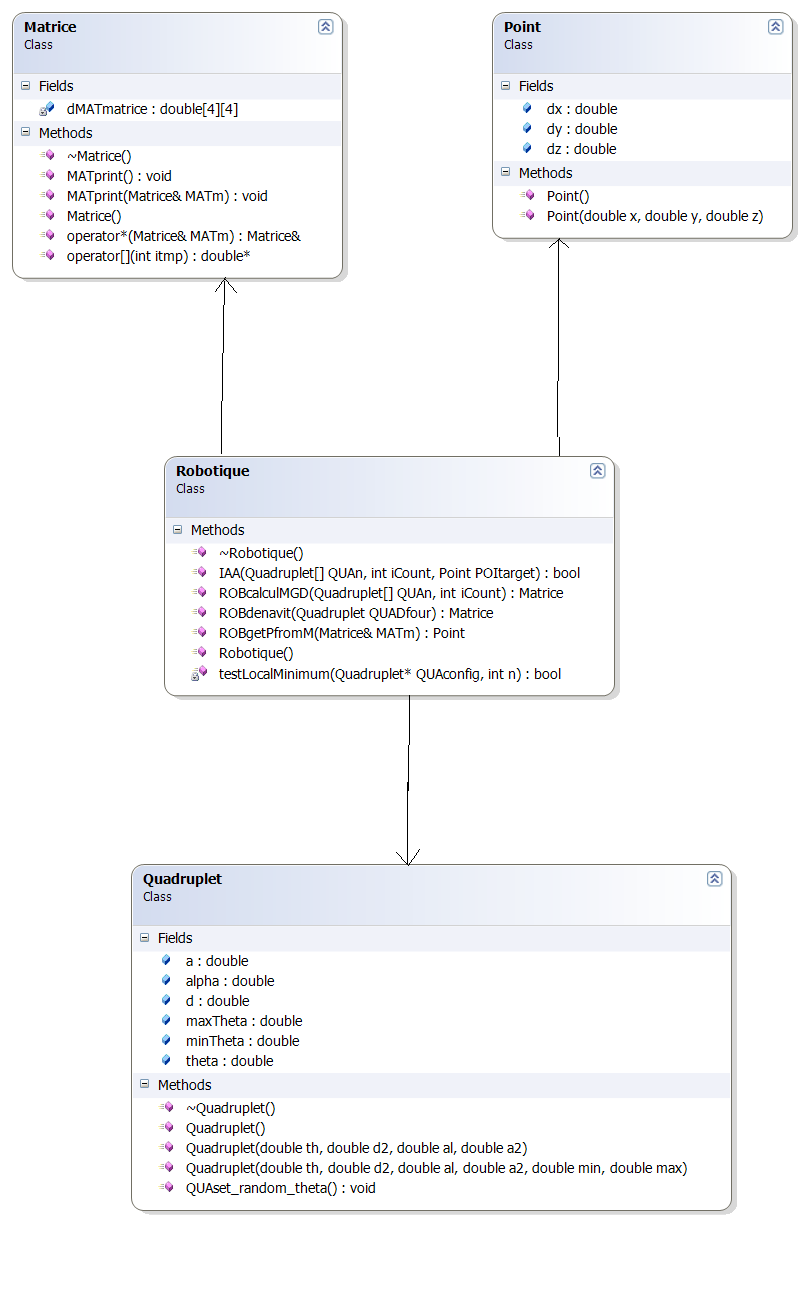
\includegraphics[scale=0.7]{pics/ch2_classdiagram.png}
	\caption{Diagramme de classes}
	\label{fig:ch2_classdiagram}
\end{figure}

%\begin{center}
%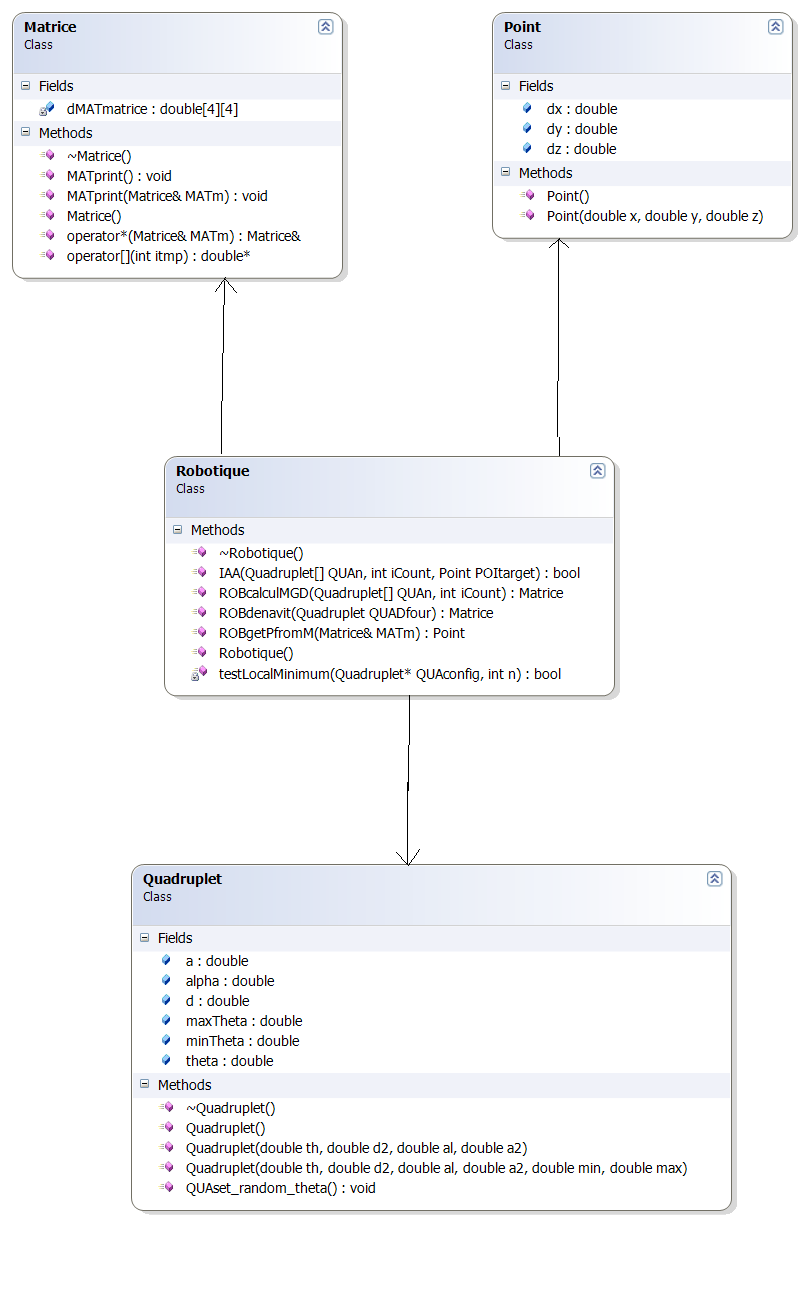
\includegraphics{pics/ch2_classdiagram.png}%
%\captionof{figure}{text}\label{labelname}%
%\end{center}

\subsection{Le code source critique de l'algorithme}
Dans cette section, nous mettons le code source de la fonction critique qui r�alise l'algorithme IAA: 


\begin{lstlisting}[language=C++]
/**L'algorithme qui v�rifie si un point est atteignable. 
*@param QUAn Un tableau de quadruplet qui repr�sente la configuration du robot.
*            Les valeurs QUAn[i].theta sont � chercher, dons les valeurs initiales
*            sont ignor�s.
*@param iCount Le nombre de quadruplet dans le tableau QUAn
*@param POItarget Le point cible.
*@result false Si le point cible n'est pas atteignable
*        true  Si le point cible est atteignable, les valeurs articulaires
*              sont affect� � QUAn[i].theta.
*/
bool Robotique::IAA(Quadruplet QUAconfig[], int n, Point POItarget)
{
int i;
bool flag = true;
double lastX;//The theta of the last time
  
//A table of increment rate
double *incRate = new double[n];
  
//stop condition
double *BORNE_RATE = new double[n];
  
//The coordinate of the current point that we can reach
Point POIcurrent;
  
//The distance between the current point and the target point
double lastDist, newDist;
  
//Initialisation
for(i=0; i<n; i++)
{
    QUAconfig[i].QUAset_random_theta();
    incRate[i]=0.15;//cf the article of Abdelhak MOUSSAOUI
    
    //Stop condition: If the value of IncrementRate is less
    //than this threshold, and the values of theta cannot be
    //improved, then the function return false, which means that
    //the target point is not reachable.
    BORNE_RATE[i]=0.0001*PI/180/    //precision:0.00...1�
        (QUAconfig[i].maxTheta - QUAconfig[i].minTheta);
}

POIcurrent = ROBgetPfromM(ROBcalculMGD(QUAconfig, n));
lastDist = distance(POIcurrent, POItarget);

int j=0, times = 0;
while(flag)
{
    flag = false;
    
    //for each value of theta
    for(i=0; i<n; i++)
    {
        POItarget.dx, POItarget.dy, POItarget.dz);
        lastX = QUAconfig[i].theta;
        
        //inc
        QUAconfig[i].theta+=(QUAconfig[i].maxTheta-QUAconfig[i].minTheta)*incRate[i];
        if(QUAconfig[i].theta > QUAconfig[i].maxTheta)
            QUAconfig[i].theta = QUAconfig[i].maxTheta;

        POIcurrent = ROBgetPfromM(ROBcalculMGD(QUAconfig, n));
        newDist = distance(POIcurrent, POItarget);
                 
        if (newDist < lastDist)
        {//We get a better value
          //Keep the new value
          lastDist=newDist;
          flag=true;
        }
        else
        {
            //search another possibility
		        QUAconfig[i].theta = lastX - 
		          (QUAconfig[i].maxTheta-QUAconfig[i].minTheta)*incRate[i];
            if(QUAconfig[i].theta < QUAconfig[i].minTheta)
                QUAconfig[i].theta=QUAconfig[i].minTheta;
                
            //calculate new distance
            POIcurrent = ROBgetPfromM(ROBcalculMGD(QUAconfig, n));
	          newDist = distance(POIcurrent, POItarget);
            if(newDist < lastDist)
            {//We get a better value
                //Keep the new value
                lastDist = newDist;
                flag = true;
            }
            else
            {
                //Keep the original value
                QUAconfig[i].theta=lastX;
                
                //Adjust increment rate
                incRate[i]/=2;
                if(incRate[i]>BORNE_RATE[i])
                   flag = true;
                newDist = lastDist;
            }
              
        }
        if(newDist<BORNE_DIS)
        {
            delete []incRate;
            return true;
        }
    }
}

    if(true == testLocalMinimum(QUAconfig, n))
    {
        printf("We've probably encountered a \"Local minimum\" situation. Try again.\n");
    }
    delete []incRate;
    return false;
}
\end{lstlisting}


\section{Test de l'algorithme IAA}
Apr�s avoir fini le codage de l'algorithme, nous l'avons test� avec quelques exemples de robots qu'on a vus dans les cours de la robotique. 

\subsection{Un exemple sp�cifique}
Nous pr�sentons un exemple sp�cifique que nous avons test�, concernant un manipulateur de 5 rotations, repr�sent� dans la figure au-dessous:


\begin{figure}[!htbp]
	\centering
		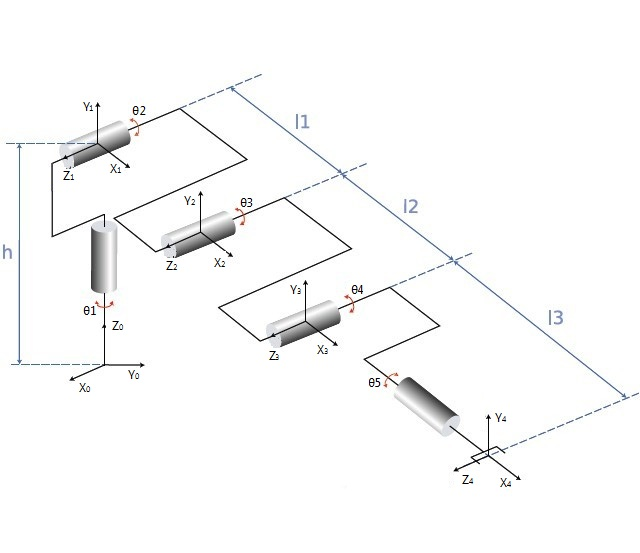
\includegraphics[scale=0.6]{pics/ch2_config.jpg}
	\caption{Le med�le utilis� (h=2m; l1,l2,l3=1m)}
	\label{fig:ch2_config}
\end{figure}


Selon notre impl�mentation, pour repr�senter cette configuration du bras manipulateur, il suffit de cr�er un tableau d'objet de classe \textbf{Quadruplet}, dont chaque objet repr�sente une transformation de rep�re. La derni�re articulation est particuli�re, elle n'intervient pas dans notre travail, car la rotation de cette articulation ne change pas les coordonn�es du point de l'organe terminal. Donc on a 4 objets au total dans le tableau:

\begin{lstlisting}[language=C++]
//La r�pr�sentation de la configuration du bras manipulateur (On a impos� des limites)
Quadruplet pQUAconfig1[4];
pQUAconfig1[0] = Quadruplet(PI/2, 2, PI/2, 0,     0,   PI);
pQUAconfig1[1] = Quadruplet(   0, 0,    0, 1, -PI/2, PI/2);
pQUAconfig1[2] = Quadruplet(   0, 0,    0, 1,     0, PI/2);
pQUAconfig1[3] = Quadruplet(   0, 0,    0, 1,     0, PI/2);

//La repr�sentation du point cible � tester
Point POItarget1(0,0,3);
\end{lstlisting}

\bigskip
Et puis on peut appeler la fonction IAA:
\begin{lstlisting}[language=C++]
//La valeur renvoy�e indique si le point cible est bien atteignable ou non.
bool res = Robotique::IAA( pQUAconfig1, 4, POItarget1);

//C'est une fonction d�finie pour afficher les valeurs des
//variables articulaires.
printResIAA(pQUAconfig1, 4, res);
\end{lstlisting}

\clearpage
\subsection{Interpr�tation de la solution}
En cons�quence de cet exemple sp�cifique, nous avons obtenu dans la fen�tre de terminal:

\begin{figure}[!htbp]
	\centering
		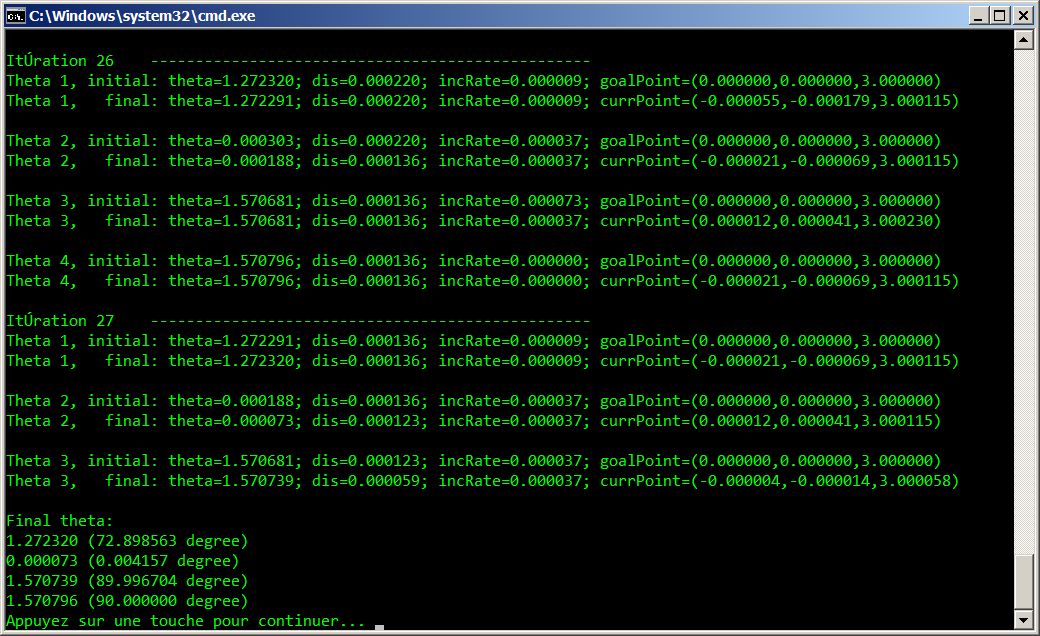
\includegraphics[scale=0.5]{pics/ch2_result.png}
	\caption{R�sultat obtenu}
	\label{fig:ch2_result}
\end{figure}


L'algorithme a pass� 27 it�rations pour trouver la solution. Les valeurs des 4 variables articulaires finales sont affich�es � la fin. Cette solution peut �tre interpr�t�e comme ceci: pour atteindre le point (0,0,3), les 4 angles de rotation $\Theta_1,\Theta_2,\Theta_3,\Theta_4$ sont respectivement 73�,0�,90�,90�. Il peut aussi y avoir des autres solutions possibles. 

\chapter{Difficult�s rencontr�es}
\section{Probl�mes r�solus}
\subsection{Probl�me sur la pr�cision}
Au d�but de l'impl�mentation de l'algorithme, nous obtenions souvent des r�sultats d�raisonnables. Apr�s avoir discut� avec notre encadrant, nous nous sommes aper�us que �a soit un probl�me de pr�cision. �a concerne la repr�sentation interne des donn�es en C++. Et puis nous avons chang� notre type de donn�e � \textbf{double} qui a enfin r�solu ce probl�me.


\section{Probl�mes non r�solus}
\subsection{Probl�me des minimums locaux}
Un avantage de l'algorithme IAA est qu'on peut imposer des limits sur les variables articulaires, pour que la solution respecte certains crit�res particuliers. Mais �a nous am�ne aussi le probl�me des minimums locaux. Parfois l'algorithme se converge vers un minimum local (mais pas global), et donc dans un �tat consistant. En cons�quence, il nous dit qu'il y a pas de solution (le point cible n'est pas atteignable), mais le point est en fait atteignable, et la solution n'�tait pas trouv�e � cause des minimums locaux.


C'est un probl�me commun des algorithmes similaires. C'est � cause des limites qu'on a impos�es aux variables articulaires et � la initialisation al�atoire d'elles. Nous ne pouvons pas �liminer ce probl�me, mais nous pouvons essayer de l'examiner, pour qu'on puisse relancer l'algorithme au lieu de croire qu'il n'y a pas de solution.


Nous constatons que quand un "minimum local" appara�t, il y a au moins une variable articulaire qui a atteint sa limite qu'on l'a impos�e. Selon �a, dans notre programme, si aucune solution n'est trouv�e, on va tester les variables articulaires courantes, s'il existe une variable articulaire qui a atteint sa limite, alors on affiche un message disant qu'on a \textbf{probablement} rencontr� un minimum local. � savoir qu'on ne l'a pas prouv� mais plut�t le tester selon les exp�riences.

\begin{figure}[!ht]
	\centering
		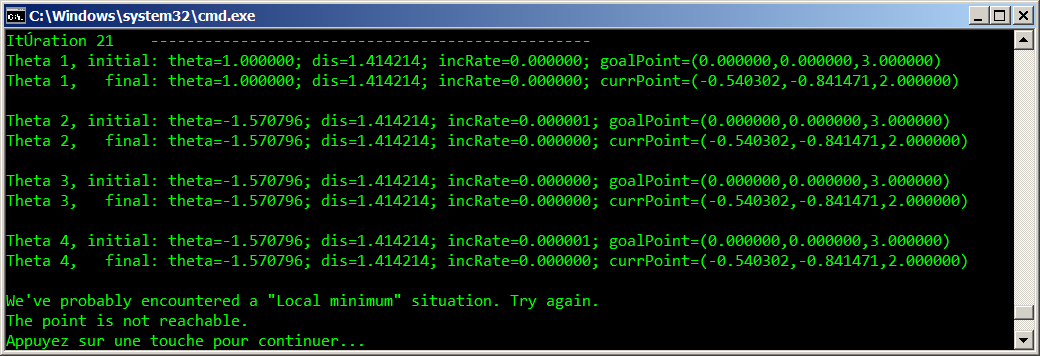
\includegraphics[scale=0.4]{pics/ch3_localminimum.png}
	\caption{Message affich� quand un minimum local appara�t}
	\label{fig:ch3_localminimum}
\end{figure}

\subsection{Probl�me de vitesse de convergence}
La vitesse de convergence est aussi un probl�me de cet algorithme, surtout quand le point cible est sur la fronti�re de la zone atteignable du bras manipulateur. En ce cas particulier, l'algorithme peut enfin trouver la solution, mais la vitesse de convergence devient tr�s lente quand l'organe terminal approche du point cible.



%
\chapter{Conclusion}
Notre projet concerne la compr�hension, impl�mentation et le test d'un l'algorithme(IAA) qui peut v�rifier l'accessibilit� d'un point dans l'espace par un bras manipulateur. Nous commencions notre travail par la lecture de deux articles propos�s par notre encadrant. Apr�s avoir compris l'algorithme, nous l'avons impl�ment� en C++, et l'avons test� avec quelques exemples de bras manipulateur qu'on a vu en cours.


Ce projet nous a renforc� la compr�hension sur la cin�matique robotique, surtout le \textit{Mod�le G�om�trique Direct} et le \textit{Mod�le G�om�trique Inverse}. �a nous permet aussi d'avoir une impression sur l'application de robotique dans la vie r�elle.

\begin{thebibliography}{9}
   \bibitem{1}
          Otmani R., 
          Pruski A.,
          Belarbi K.,
          \emph{La r�alit� virtuelle comme outil pour l'�valuation, la visualisation et la validation de l'accessibilit� d'un lieu de vie}.
          Conf�rence Handicap 2010,
          juin 2010,
          Paris.
    \bibitem{2}
    			Abdelhak MOUSSAOUI,
    			\emph{Prise en charge de psychotherapie et du handicap par la r�alit� virtuelle}.
    			UNIVERSIT� ABOU BEKR BELKA�D-TLEMCEN FACULTE DE TECHNOLOGIE,
    			30 juin 2012.

\end{thebibliography}
\annexes

\end{document}

